\documentclass[./00PhotoBox.tex]{subfiles}
\graphicspath{{\subfix{./img/}}}
\begin{document}

\chapter{Untersuchungen zur Genauigkeit und Systemaufbau}
Nach Abschluss der Konstruktion und des Aufbaus des Prototyps, wurden verschiedene Untersuchungen durchgeführt, um die Genauigkeit des Systems zu überprüfen und die Anzahl der Kameras zu evaluieren. Hierzu wurden unter anderem Vergleichsmessungen mit verschiedenen Systemen durchgeführt.

\section{Genauigkeitsüberprüfung des 3D-Modelles}
\label{s:genauigkeitsueberpruefung}
Um die Genauigkeit der 3D-Modell-Erzeugung zu überprüfen, wurden mehrere Prüfkörper mit dem Prototypen und mit einem kommerziellen Streifenprojektionssystem vermessen. Die Ergebnisse wurden miteinander verglichen.

\subsection{Erwartete Genauigkeit}
\label{ss:erwartete_genauigkeit}
Die erwartete Genauigkeit kann auf verschiedenen Wegen berechnet werden. Grundlage ist meistens der Bildmaßstab. Dieser unterscheidet sich je nach Entfernung. Die Entfernung zum Objekt beträgt im Normalfall zwischen 10 und 50~cm. Der Bildmaßstab $m$ berechnet sich nach \cite[S. 171]{luhmann} wie folgt:

\begin{align}
    m       & = \frac{h}{c}                                  \\
    m_{min} & = \frac{100~\text{mm}}{4,7~\text{mm}} = 21,28  \\
    m_{max} & = \frac{500~\text{mm}}{4,7~\text{mm}} = 106,38
\end{align}

Für die Bildmessgenauigkeit werden verschiedene Werte in der Literatur erwähnt, sie liegen je nach Messmethode zwischen 0,05 und 3~px. Für Messung von CCCTs wird z.B. von \cite{soot2015} eine Genauigkeit von 0,1~px angegeben.
Eigene, manuelle Messungen ergaben eine Genauigkeit von etwa 1,5~px. Vereinfacht wurde mit 1~px Genauigkeit gerechnet.

\begin{align}
    dx'      & = 1~\text{px} = 0,0014~\frac{\text{mm}}{\text{px}} \cdot 12~\text{px} = 0,0014~\text{mm} \\
    dX       & = m \cdot dx'                                                                            \\
    dX_{min} & = 21,28 \cdot 0,0014~\text{mm} = 0,03~\text{mm}                                          \\
    dX_{max} & = 106,38 \cdot 0,0014~\text{mm} = 0,15~\text{mm}
\end{align}

An diesem Wert muss dann noch der sogenannte Design-Faktor angebracht werden, dieser liegt bei Rundumverbänden zwischen 0,4 und 0,8, bei Stereoaufnahmen bei 1,5-3,0 \citep[S. 174]{luhmann}. Vereinfacht für eine grobe Abschätzung wird hier daher der Faktor weggelassen. Die erwartete Genauigkeit liegt damit deutlich unter einem Millimeter in der Lage.

\begin{align}
    s_{px; min}' & = dX_{min} \\
    s_{px; max}' & = dX_{max}
\end{align}

Die Genauigkeit der Tiefeninformationen ist von dem Verhältnis des Abstandes der Kameras zur Entfernung abhängig. Zwischen zwei Kamerareihen sind etwa 25~cm Abstand. Die Genauigkeit der Tiefeninformationen kann daher wie folgt berechnet werden \citep[S. 174]{luhmann}:

\begin{align}
    s_Z       & = m \cdot \frac{h}{b} \cdots s_{px}'                                                   \\
    s_{Z;min} & = 21,28 \cdot \frac{10~\text{cm}}{30~\text{cm}}\cdot 0,03~\text{mm}  = 0,02~\text{mm}  \\
    s_{Z;max} & = 106,38 \cdot \frac{50~\text{cm}}{30~\text{cm}} \cdot 0,15~\text{mm} = 0,25~\text{mm}
\end{align}

Die erwartete Genauigkeit und auch die Auflösung der Kameras liegt also im Bereich eines Fünftel Millimeters.


\subsection{Vergleichsmessung mit Streifenprojektionssystem}
Als Vergleichsmessung wurden die Objekte mit einem Zeiss GOM ATOS 5 aufgemessen. Hierbei handelt es sich um ein Streifenprojektionssystem, welches hauptsächlich in der Industrie zur Vermessung von Bauteilen eingesetzt wird. Streifenprojektionssysteme arbeiten auch photogrammetrisch, haben aber den Vorteil, das sie durch das Projektionssystem auch texturarme Objekte erfassen können. Wie der Name bereits andeutet, wird ein Streifenmuster auf das Objekt projiziert, welches dann von mindestens einer Kamera aufgenommen wird. Projektor und Kamera sind auf einer festen Basis montiert. \citep[S. 581f]{luhmann}

Bei dem verwendeten System werden zwei Kameras eingesetzt, die sich ein massives Gehäuse mit dem mittig angeordneten Projektor teilen. Bei dem verwendeten Messvolumen und Objektentfernung beträgt die Genauigkeit etwa \todo{Wert}. Aufgrund der deutlich höheren erwarteten Genauigkeit des Streifenprojektionssystems, kann davon ausgegangen werden, dass die Messungen deutlich genauer sind als die des Prototypen und als wahre Werte angenommen werden können.

\subsection{Ergebnisse}
Die modellierte Oberfläche aus dem Streifenprojektionssystem und die Punktwolke aus dem Prototypen wurden in CloudCompare aufeinandergelegt und die Differenz berechnet. Die Visualisierung der Differenzen ist in \autoref{fig:differenz_moia} dargestellt. Es ist zu erkennen, dass einige Bereiche gar nicht erfasst bzw. deren Genauigkeit deutlich von der erwarteten abweichen. Die größten Fehlstellen sind im Bereich des Kinnes und unterhalb des Bauches zu erkennen. Die Abweichungen im Bereich des restlichen Körpers sind deutlich geringer und liegen im Bereich von 0,21~mm. Die Abweichungen sind auf die schlechtere Erfassung der nach unten gerichteten Flächen \todo{andere Beschreibung oder Fehler vermeiden} zurückzuführen. Diese Bildbereiche sind nur in wenigen Bildern sichtbar und können daher nicht so gut rekonstruiert werden.

Die Abweichungen liegen in der Größenordnung der in \autoref{ss:erwartete_genauigkeit} berechneten Werte und sind nur minimal schlechter, als die Genauigkeit eines 3D-Modelles des Körpers, welches photogrammetrisch mit einer Spiegelreflexkamera Nikon D90 manuell aufgenommen wurde. Durch Kombinationen von anderne Perspektiven ist hier jedoch die Abdeckung, welche hier nicht objektiv betrachtet wurde, besser. Die Ergebnisse sind in \autoref{tab:vergleich_erg} zusammengefasst.

\begin{figure}
    \centering
    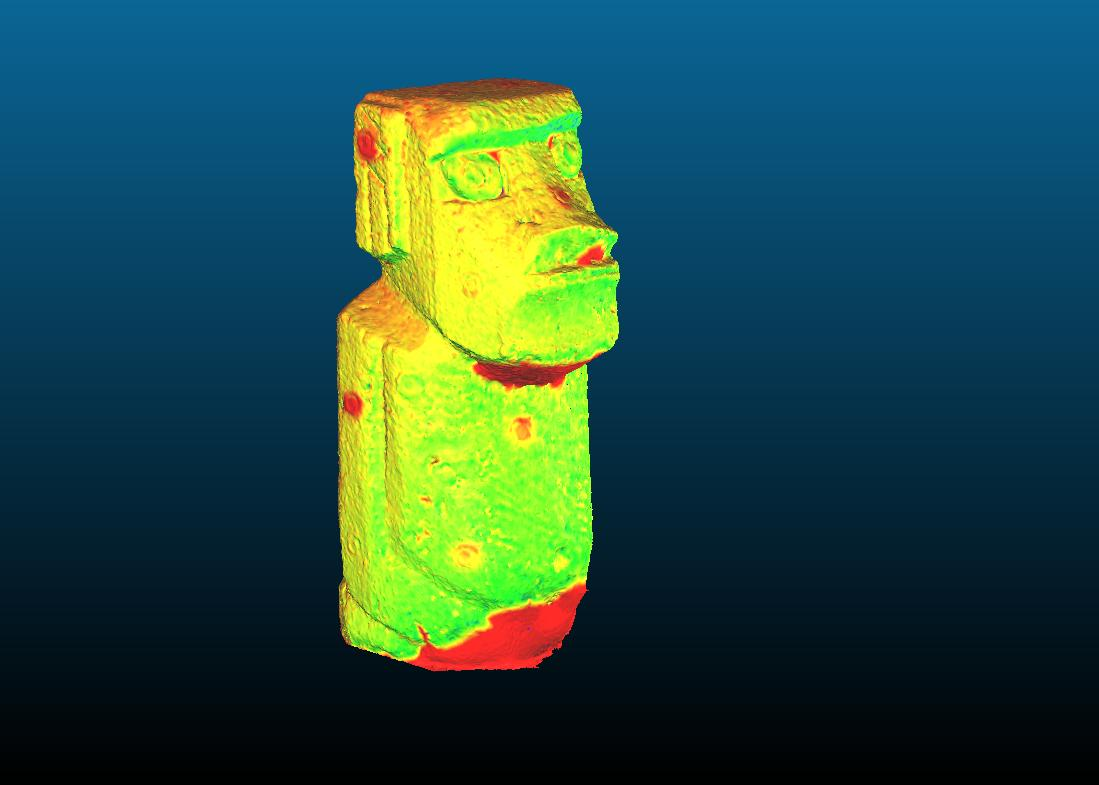
\includegraphics[width=0.8\textwidth]{img/moai_fehler.jpg}
    \caption{Differenzbild des Moai (rot: Fehler größer 0,5 mm)}
    \label{fig:differenz_moia}
\end{figure}

\begin{table}
    \centering
    \caption{Ergebnisse der Genauigkeitsüberprüfung}
    \label{tab:vergleich_erg}
    \begin{tabular}{l|r|r|r}
        \toprule
                   & Durchschnittliche & Mittlerer & Maximaler \\
                   & Fehler            & Fehler    & Fehler    \\
        \midrule
        Gesamt     & 0,37~mm           & 1,09~mm   & 11,6~mm   \\  % Oberflächenmodell alt
        gefiltert  & 0,20~mm           & 0,72~mm   & 1,9~mm    \\
        \midrule
        Punktwolke & 0,04~mm           & 0,21~mm   & 3,3~mm    \\  % Vertices neu
        \midrule
        Nikon D90  & 0,27~mm           & 0,19~mm   & 1,2~mm    \\
        \bottomrule
    \end{tabular}
\end{table}


\section{Evaluation der Kameraanzahl}
Zur Abschätzung, wie viele Kameras für eine gute Genauigkeit notwendig sind, wurden verschiedene Konfigurationen getestet. Hierzu wurde die Aufnahme des Moai aus \autoref{s:genauigkeitsueberpruefung} genutzt und hier in Agisoft Metashape verschiedene Kameras deaktiviert und das 3D-Modell neu berechnet. Die Ergebnisse wurden wie \autoref{s:genauigkeitsueberpruefung} mit dem Streifenprojektionssystem verglichen.
\todo{Ergebnisse}


\section{Nutzung eines Drehtellers}
Statt die reele Zahl der Kameras zu verändern, kann auch ein Drehteller genutzt werden, so dass jede Kamera mehr als ein Bild zur Erfassung des Objektes liefert.

\subsection{Durchführung}
Hierzu wurde ein einfacher manueller Drehteller genutzt (IKEA SNUDDA). Dieser wurde mit Passpunkten beklebt und weißt ansonsten eine texturreiche Naturholzoberfläche auf (siehe \autoref{fig:drehteller_moai}). Die Daten würde in Metashape weiterverarbeitet und die einzelnen Aufnahmeschritte über die Passpunkte und die Punktwolke zusammengerechnet. Die Ergebnisse wurden mit denen des Streifenprojektionssystems und den Aufnahmen ohne Drehteller verglichen.

\begin{figure}
    \centering
    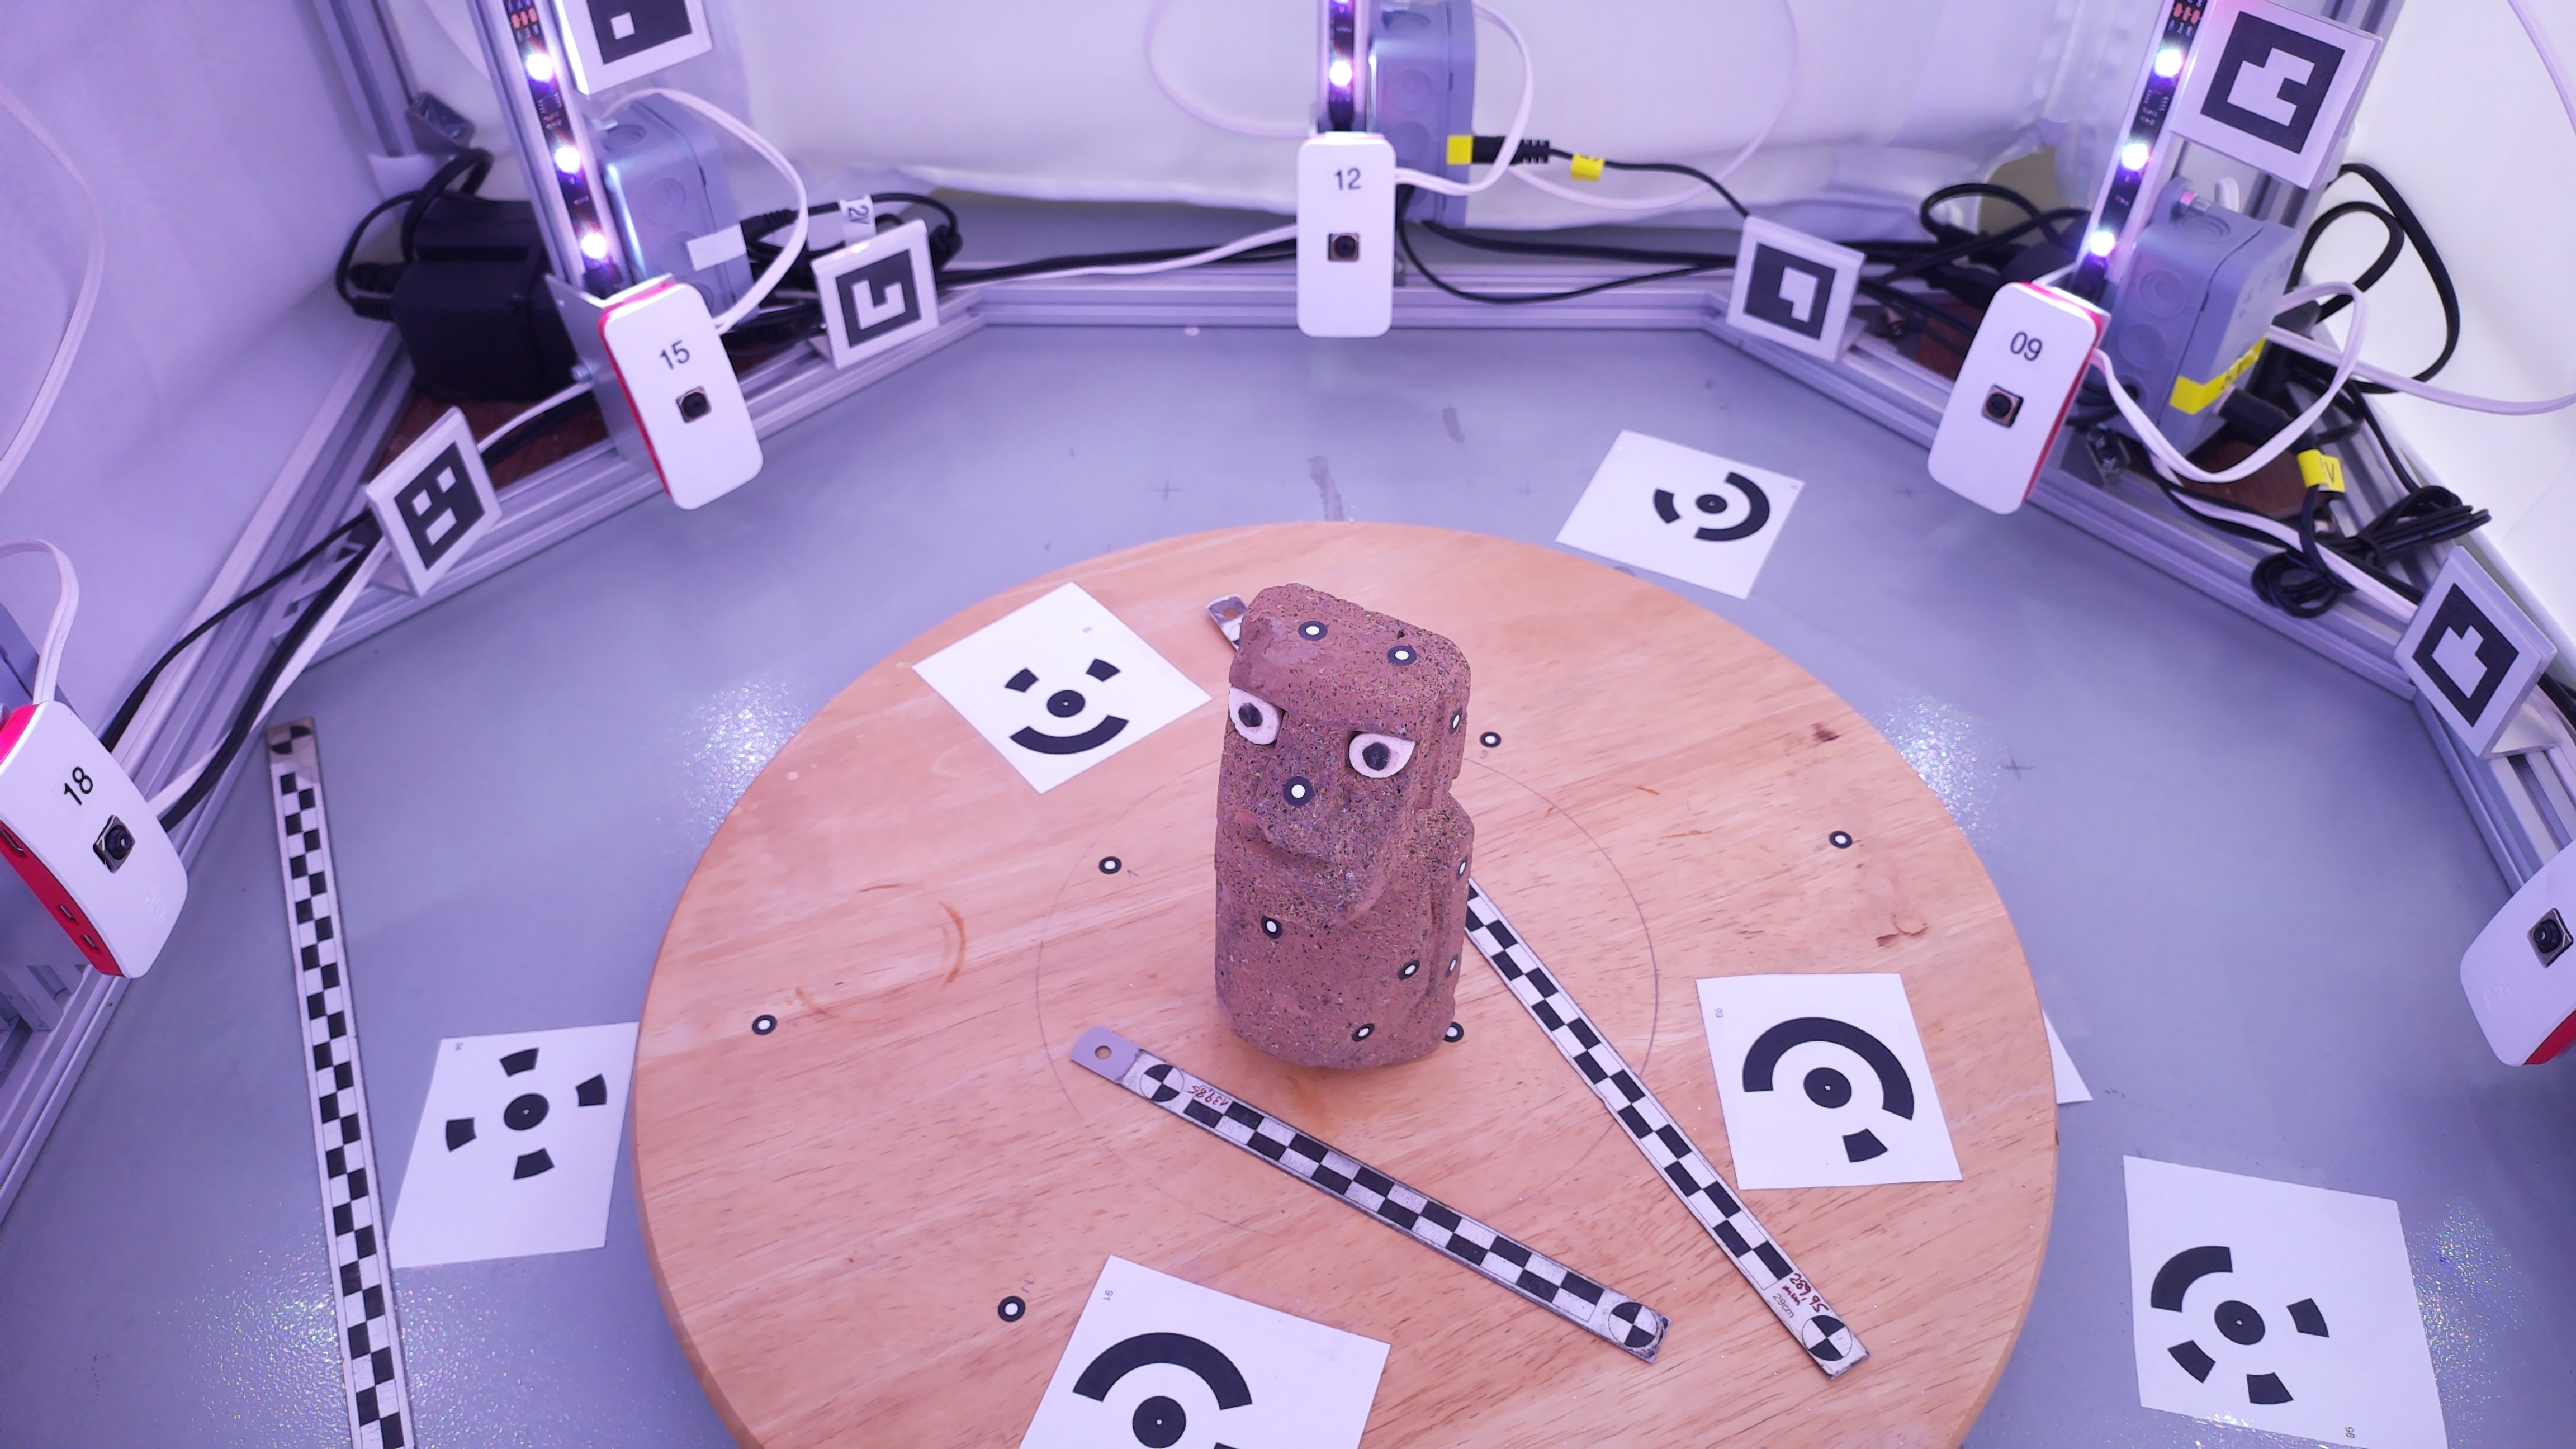
\includegraphics[width=0.8\textwidth]{img/drehteller_moai.jpg}
    \caption{Drehteller mit Moai-Figur im Prototypen (aufgenommen von einem der verbauten Raspberry Camera Module v3)}
    \label{fig:drehteller_moai}
\end{figure}

\subsection{Ergebnisse}

\begin{table}
    \centering
    \caption{Ergebnisse der unter Anpassung des Maßstabes durchgeführten Genauigkeitsüberprüfung}
    \label{tab:vergleich_drehteller}
    \begin{tabular}{l|r|r|r|r}
        \toprule
                        & Durchschnittliche & Mittlerer & Maximaler & Punktanzahl \\
                        & Fehler            & Fehler    & Fehler    &             \\
        \midrule
        ohne Drehteller & - 0,03~mm         & 0,22~mm   & 2,0~mm    & 3,3 Mio     \\
        mit Drehteller  & - 0,03~mm         & 0,15~mm   & 1,6~mm    & 3,4 Mio     \\
        Nikon D90       & 0,03~mm           & 0,17~mm   & 1,2~mm    & 0,05 Mio    \\
        \bottomrule
    \end{tabular}
\end{table}
\todo{Auswerten}

\begin{figure}
    \centering
    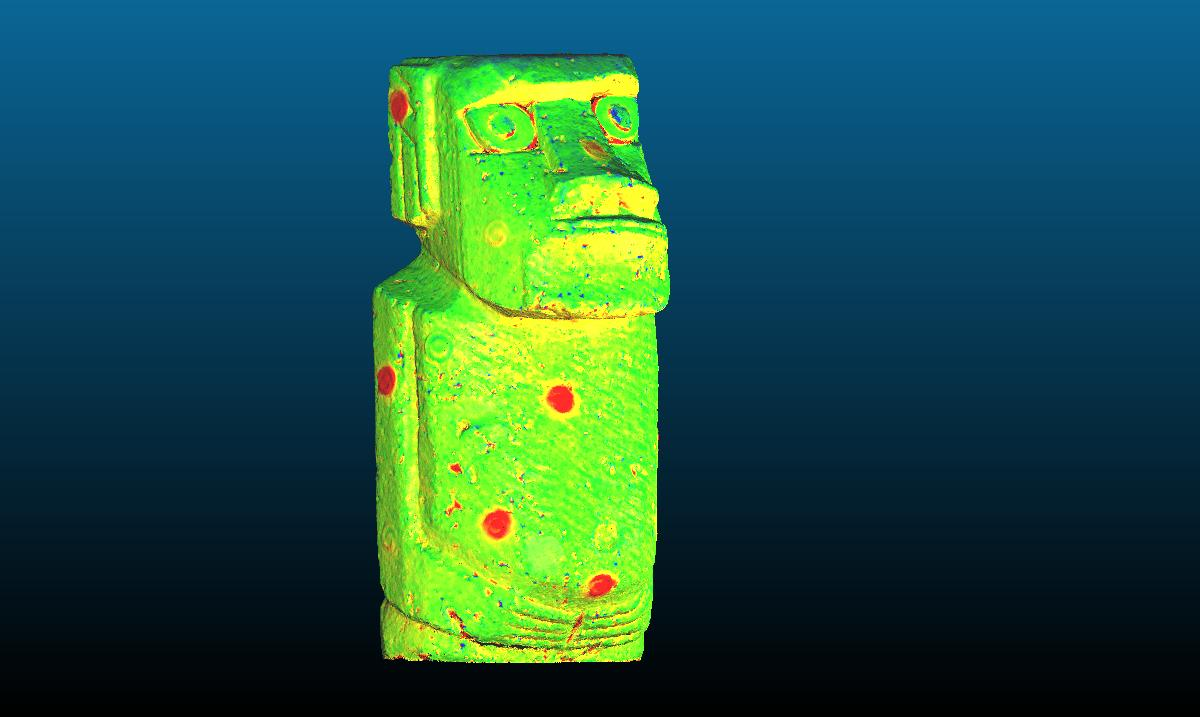
\includegraphics[width=0.8\textwidth]{img/moai_fehler_drehteller.jpg}
    \caption{Differenzbild des Moai (rot: Fehler größer 0,5 mm)}
    \label{fig:drehteller_moai_fehler}
\end{figure}

\biblio
\end{document}